\documentclass{rapportENIAD}

% Configuration and Packages
%----------------------------------------------------------------------------------------
%	PACKAGES AND OTHER DOCUMENT CONFIGURATIONS
%----------------------------------------------------------------------------------------

\usepackage{lipsum}
\usepackage[table]{xcolor}
\usepackage{minted}
\definecolor{bg}{rgb}{0.95,0.95,0.95} % Adjust the RGB values as needed
\usepackage{titlesec} % For customizing chapter and section titles
\usepackage{tocloft} % For customizing the table of contents
\usepackage{hyperref} % For adding hyperlinks
\usepackage{setspace} % For line spacing adjustments

\graphicspath{{figures/}{logos/}}


% Document Metadata
%----------------------------------------------------------------------------------------
%	DOCUMENT INFORMATION
%----------------------------------------------------------------------------------------

\title{Rapport - HR Analytics - Employee Attrition \& Performance}

\titre{HR Analytics - Employee Attrition \& Performance}
\UE{} % Nom de l'Unité d'Enseignement
\sujet{Projet de Fin de Module}

\enseignant{M. Mohamed BADIY}

\eleves{
    Zakariae EL HADDOUCHI \\
    Meryame EL AIBOUDI \\
    Oussama LEBYED \\
    Oualid BOUTAYEB
}

\jury{}


\begin{document}

%----------- Initialisation -------------------
\fairemarges % Afficher les marges
\fairepagedegarde % Créer la page de garde

%-------------- Front Matter --------------
\pagenumbering{roman} % Page numbering in Roman numerals for front matter

\chapter*{Remerciements}
\addcontentsline{toc}{chapter}{Remerciements}

\begin{center}
    
\includegraphics[width=0.4\textwidth]{logos/motif decoratif haut.PNG}
\end{center}

\vspace{0.5cm}

\begin{onehalfspace}
Au terme de ce projet de Business Intelligence, nous tenons à exprimer notre profonde gratitude à toutes les personnes qui ont contribué à son bon déroulement et à son aboutissement.

Nous adressons nos remerciements les plus sincères à notre enseignant et encadrant, \textbf{M. Mohamed BADIY}, pour ses conseils précieux, son orientation constante et la qualité de son enseignement tout au long de ce module. Son expertise et sa disponibilité ont été des atouts majeurs dans la réalisation de ce travail.

Nos remerciements vont également à l'ensemble du corps professoral de l'École Nationale de L'Intelligence Artificielle et du Digital (ENIAD) pour la richesse du programme académique et pour nous avoir fourni les outils théoriques et pratiques nécessaires à notre formation de futurs experts de la donnée.

Enfin, nous tenons à remercier nos familles et nos amis pour leur soutien moral et leurs encouragements constants, qui ont été une source de motivation indispensable tout au long de ce parcours.
\end{onehalfspace}

\vspace{0.5cm}

\begin{center}
    
\includegraphics[width=0.4\textwidth]{logos/motif decoratif bas.PNG}
\end{center}

\chapter*{Résumé}
\addcontentsline{toc}{chapter}{Résumé}

\begin{onehalfspace}
Ce projet présente la conception et la mise en œuvre d'une solution de Business Intelligence (BI) dédiée à l'analyse de l'attrition et de la performance des employés. L'objectif principal est d'identifier les facteurs déterminants qui influencent le départ des collaborateurs au sein d'une organisation afin de proposer des stratégies de rétention basées sur les données. En s'appuyant sur un jeu de données de ressources humaines comprenant 1470 observations, nous avons déployé une architecture décisionnelle complète. La méthodologie adoptée comprend une phase d'exploration des données (EDA), la conception d'un modèle dimensionnel en étoile optimisé pour les analyses RH, ainsi qu'un processus ETL rigoureux pour le nettoyage et la transformation des informations. Les résultats, présentés sous forme de tableaux de bord interactifs, mettent en évidence l'impact prépondérant des heures supplémentaires, du niveau de rémunération et de l'équilibre vie-travail sur la stabilité des effectifs. Ce travail offre une base analytique solide pour orienter les politiques de gestion des talents et ouvre la voie à l'utilisation de modèles prédictifs pour anticiper les risques d'attrition.

\textbf{Mots-clés :} Business Intelligence, HR Analytics, Attrition, Modélisation dimensionnelle, ETL, Visualisation de données.
\end{onehalfspace}

\chapter*{Abstract}
\addcontentsline{toc}{chapter}{Abstract}

\begin{onehalfspace}
This project focuses on the design and implementation of a Business Intelligence (BI) solution for analyzing employee attrition and performance. The primary objective is to identify key factors influencing employee turnover and to provide data-driven retention strategies. Utilizing an HR dataset of 1470 records, we developed a comprehensive decision-support architecture. The methodology encompasses exploratory data analysis (EDA), a star-schema dimensional model optimized for HR metrics, and a robust ETL process for data cleansing and transformation. The findings, delivered through interactive dashboards, highlight the significant impact of overtime, compensation levels, and work-life balance on workforce stability. This work provides a solid analytical foundation for guiding talent management policies and paves the way for the integration of predictive models to proactively manage attrition risks.

\textbf{Keywords:} Business Intelligence, HR Analytics, Employee Attrition, Dimensional Modeling, ETL, Data Visualization.
\end{onehalfspace}

\chapter*{Liste des abréviations}
\addcontentsline{toc}{chapter}{Liste des abréviations}

\begin{description}
    \item[BI] Business Intelligence (Informatique Décisionnelle)
    \item[ETL] Extract, Transform, Load (Extraction, Transformation, Chargement)
    \item[DW] Data Warehouse (Entrepôt de Données)
    \item[RH] Ressources Humaines
    \item[KPI] Key Performance Indicator (Indicateur de Performance Clé)
    \item[EDA] Exploratory Data Analysis (Analyse Exploratoire des Données)
    \item[OLAP] Online Analytical Processing
    \item[OLTP] Online Transactional Processing
    \item[SQL] Structured Query Language
    \item[3NF] Third Normal Form (Troisième Forme Normale)
\end{description}

\chapter*{Liste des Figures}
\addcontentsline{toc}{chapter}{Liste des Figures}

\listoffigures % Utilisation de la commande standard LaTeX


% Table of Contents
\cleardoublepage
\addcontentsline{toc}{chapter}{Table des matières}
\tableofcontents
\newpage

%-------------- Main Matter --------------
\pagenumbering{arabic} % Page numbering in Arabic numerals for main content

\chapter*{Introduction générale}
\addcontentsline{toc}{chapter}{Introduction générale}

Dans le contexte actuel de la transformation digitale et de la compétitivité accrue sur le marché du travail, la gestion des ressources humaines est devenue un levier stratégique majeur pour la performance des organisations. Le capital humain, considéré comme l'atout le plus précieux d'une entreprise, nécessite une attention particulière, notamment en ce qui concerne la rétention des talents et l'optimisation de la satisfaction au travail. C'est dans cette optique que s'inscrit le domaine du \textit{HR Analytics}, une discipline qui allie la science des données et la gestion des ressources humaines pour transformer des volumes massifs d'informations en insights exploitables.

Le présent projet, intitulé \textbf{« HR Analytics - Employee Attrition \& Performance »}, a été réalisé dans le cadre du module de Business Intelligence. Son objectif principal est de concevoir et de mettre en œuvre une solution décisionnelle permettant d'analyser les facteurs déterminants de l'attrition des employés et d'évaluer les niveaux de performance au sein d'une organisation. En s'appuyant sur des données empiriques, cette étude vise à identifier les motifs récurrents de départ et à proposer des indicateurs de performance clés (KPIs) pour guider les prises de décisions managériales.

La démarche adoptée suit le cycle de vie classique d'un projet de Business Intelligence, allant de l'expression des besoins à la visualisation finale des résultats. Ce rapport est ainsi structuré en six chapitres principaux :

Le premier chapitre pose le cadre général de l'étude en présentant le contexte du projet, la problématique adressée ainsi que les objectifs visés.

Le deuxième chapitre est dédié à l'analyse fonctionnelle des besoins et à l'exploration préliminaire des données, étape cruciale pour comprendre la structure et la qualité des informations disponibles.

Le troisième chapitre expose la phase de modélisation dimensionnelle, où nous détaillerons la conception de l'entrepôt de données, notamment le schéma en étoile retenu pour cette analyse.

Le quatrième chapitre décrit le processus ETL (Extract, Transform, Load), explicitant les différentes transformations appliquées aux données pour garantir leur intégrité et leur pertinence.

Le cinquième chapitre présente les résultats de l'analyse à travers des tableaux de bord interactifs et propose une interprétation approfondie des indicateurs obtenus.

Enfin, une conclusion générale synthétise les apports du projet et ouvre des perspectives sur des évolutions futures, notamment l'intégration de modèles prédictifs.

\chapter{Cadre du Projet, Gouvernance et Analyse du Besoin}

\section{Présentation de l'Organisme d'Accueil}
Le présent projet s'inscrit dans le cadre d'une étude analytique au sein de l'École Nationale de l'Intelligence Artificielle et du Digital (ENIAD). L'objectif est de simuler une intervention de conseil en Business Intelligence pour une entreprise de services moderne faisant face à des défis de gestion de son capital humain. L'organisation cible, bien que fictive pour les besoins de l'exercice, reflète les enjeux réels des départements RH actuels : besoin de réactivité, optimisation de la rétention et pilotage par la performance.

\section{Étude de l'Existant et Critique}
Actuellement, l'entreprise gère ses données RH de manière fragmentée. Les informations sont extraites de divers systèmes (ERP, fichiers de pointage) et consolidées manuellement sous forme de classeurs Excel isolés.

\subsection{Limites identifiées}
\begin{itemize}
    \item \textbf{Processus chronophages :} La collecte et le nettoyage manuel des données occupent plus de 60\% du temps des analystes RH.
    \item \textbf{Risques d'erreurs :} Les manipulations manuelles (copier-coller, formules Excel complexes) entraînent des incohérences dans les rapports finaux.
    \item \textbf{Manque de flexibilité :} Les rapports sont statiques. Toute nouvelle demande d'analyse nécessite une refonte complète du fichier.
    \item \textbf{Absence de source unique :} Il n'existe pas de référentiel centralisé, ce qui conduit à des chiffres divergents entre les départements.
\end{itemize}

\begin{figure}[h]
    \centering
    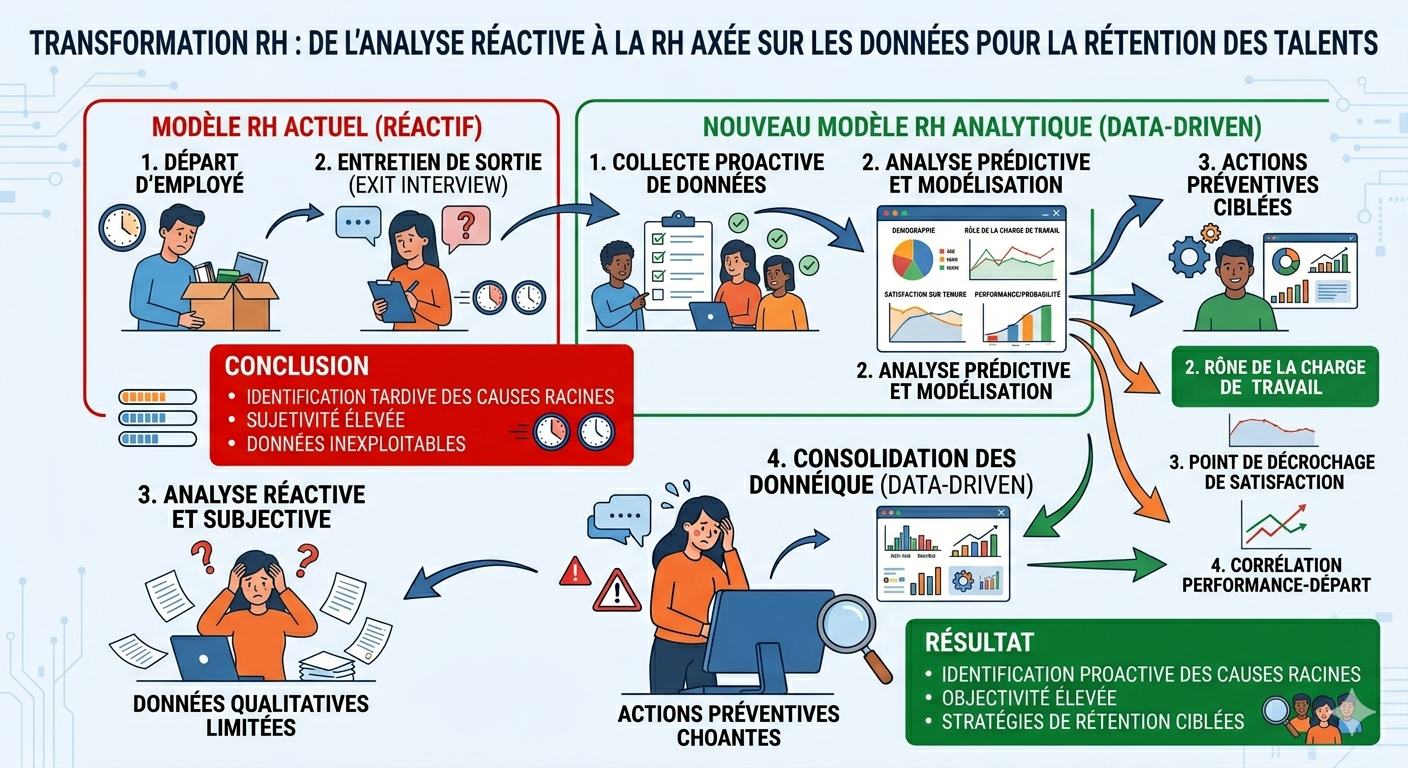
\includegraphics[width=0.8\textwidth]{figures/fig1_1_existant.png}
    \caption{Schéma de la circulation de l'information existante}
    \label{fig:existant}
\end{figure}

\section{Spécification des Besoins}

\subsection{Besoins fonctionnels}
\begin{itemize}
    \item \textbf{Calcul automatisé du Headcount :} Suivi en temps réel de l'effectif total et actif.
    \item \textbf{Analyse de l'Attrition :} Calcul dynamique du taux de départ et identification des segments à risque.
    \item \textbf{Suivi de la Satisfaction :} Corrélation entre le climat social et la rétention.
    \item \textbf{Pilotage de la Masse Salariale :} Vision globale des rémunérations par département et job role.
    \item \textbf{Filtrage dynamique :} Capacité de segmenter tous les indicateurs par période, département et genre.
\end{itemize}

\subsection{Besoins non-fonctionnels}
\begin{itemize}
    \item \textbf{Performance :} Temps de réponse des visuels inférieur à 2 secondes malgré le volume de données.
    \item \textbf{Ergonomie :} Interface intuitive respectant les codes du Data Storytelling (Thème Executive 3D).
    \item \textbf{Maintenabilité :} Architecture modulaire permettant d'ajouter de nouvelles sources facilement.
\end{itemize}

\section{Organisation de l'Équipe et Méthodologie}

Pour garantir le succès du projet, nous avons adopté une organisation par rôles spécialisés, s'appuyant sur un workflow Git rigoureux :

\begin{itemize}
    \item \textbf{Zakariae EL HADDOUCHI (Data Engineer) :} Responsable du pipeline ETL (\textit{branch: feature/etl-pipeline}). En charge de la connexion, du nettoyage et de la structuration des flux bruts.
    \item \textbf{Oussama LEBYED (Data Architect) :} Responsable de la modélisation dimensionnelle (\textit{branch: feature/data-modeling}). En charge du Schéma en Étoile et de l'intégrité des relations.
    \item \textbf{Meryame EL AIBOUDI (Business Analyst) :} Responsable de la logique analytique et documentation (\textit{branch: feature/kpi-logic}). En charge des mesures DAX et du dictionnaire de données.
    \item \textbf{Oualid BOUTAYEB (Data Visualizer) :} Responsable du design et du storytelling (\textit{branch: feature/dashboard-design}). En charge de l'UI/UX et de la restitution graphique.
\end{itemize}

\section{Planification et Suivi}
Le projet a été découpé en lots de travail suivant une approche agile. Le suivi a été assuré par un diagramme de Gantt permettant de visualiser les dépendances entre les phases ETL, Modélisation et Visualisation.

\begin{figure}[h]
    \centering
    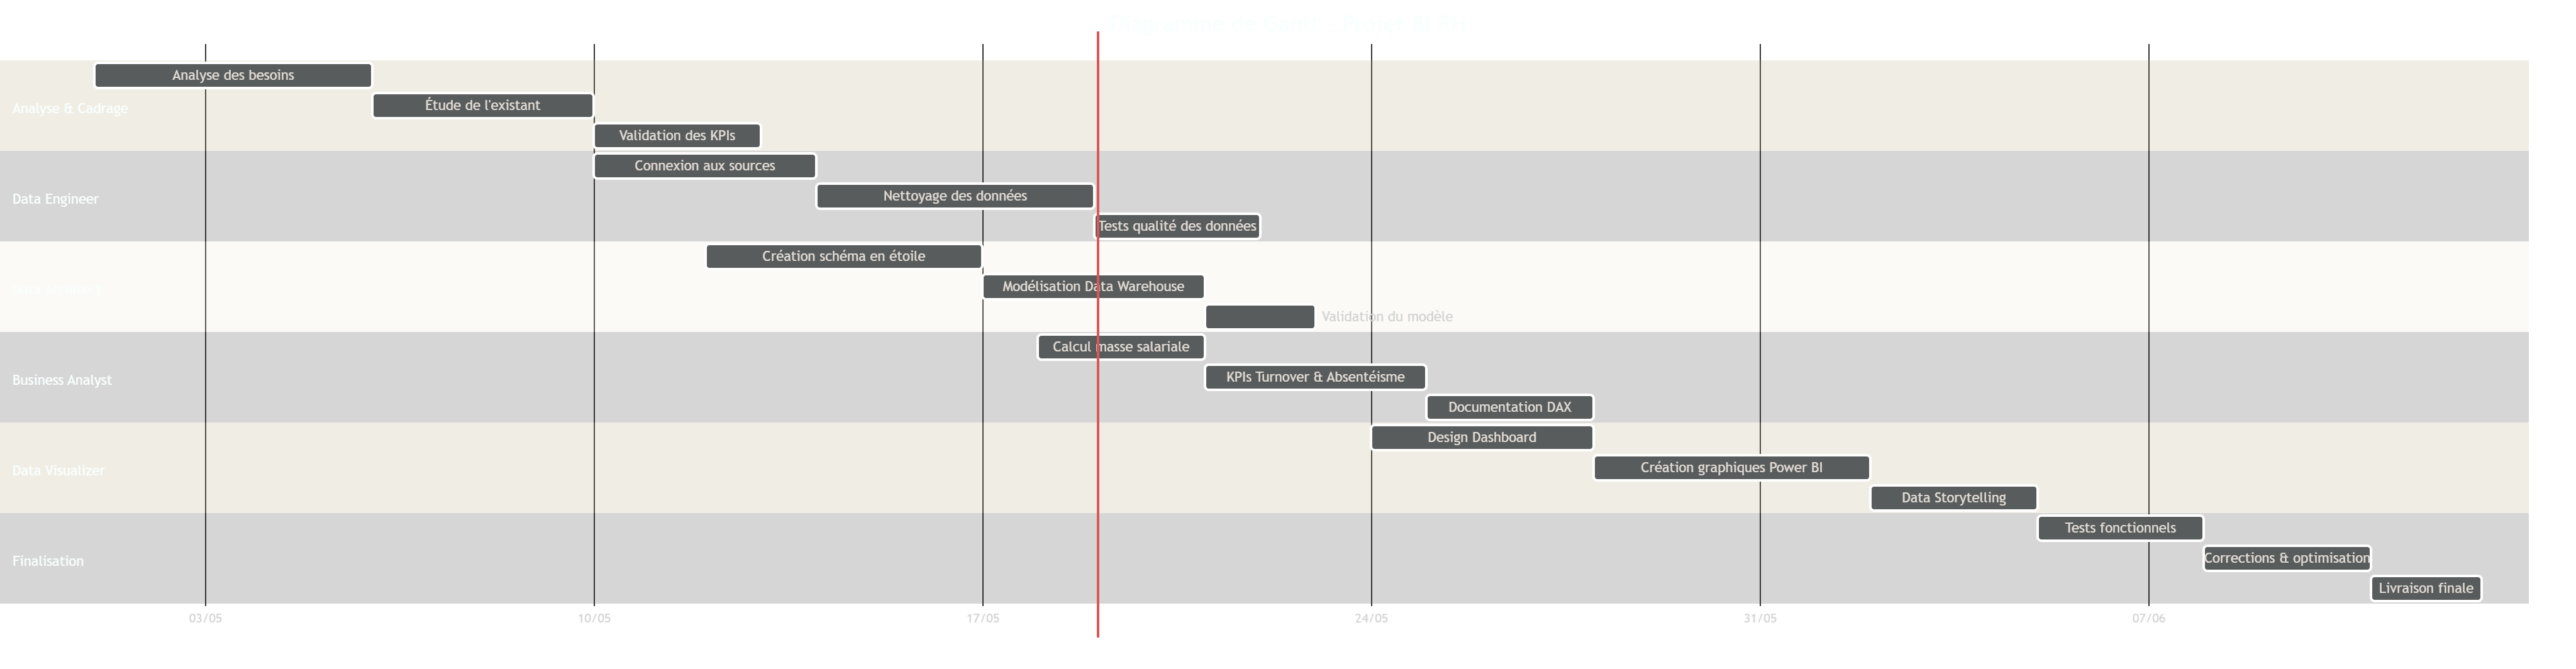
\includegraphics[width=0.8\textwidth]{figures/fig1_2_gantt.png}
    \caption{Diagramme de Gantt du projet}
    \label{fig:gantt}
\end{figure}

\chapter{Architecture Technique et Stratégie de Versioning}

\section{Fondements Théoriques de la Business Intelligence (BI)}
La Business Intelligence (BI) désigne l'ensemble des technologies et processus permettant de transformer des données brutes en informations exploitables pour la prise de décision. Le cycle de vie de la donnée dans notre projet suit les étapes classiques :
\begin{enumerate}
    \item \textbf{Collecte :} Extraction depuis les fichiers sources (CSV).
    \item \textbf{Intégration (ETL) :} Nettoyage et transformation pour assurer la qualité.
    \item \textbf{Stockage :} Organisation dans un modèle dimensionnel optimisé (Data Warehouse/Data Mart).
    \item \textbf{Analyse :} Création de mesures calculées (DAX).
    \item \textbf{Restitution :} Visualisation interactive pour les décideurs RH.
\end{enumerate}

\section{Choix de la Stack Technique et Justification}
Le choix s'est porté sur l'écosystème \textbf{Microsoft Power BI} pour plusieurs raisons stratégiques :
\begin{itemize}
    \item \textbf{Puissance du moteur VertiPaq :} Compression colonnaire permettant des performances exceptionnelles en mémoire.
    \item \textbf{Flexibilité de Power Query :} Langage M puissant pour les transformations complexes.
    \item \textbf{Richesse du DAX :} Capacité à modéliser des indicateurs métiers complexes (Time Intelligence, calculs de contexte).
    \item \textbf{Intégration :} Facilité de déploiement et de partage au sein de l'organisation.
\end{itemize}

\section{Architecture Conceptuelle de la Solution}
Pour assurer la robustesse et la maintenabilité, nous avons adopté une \textbf{architecture modulaire} en séparant les responsabilités dans trois fichiers Power BI distincts :

\begin{enumerate}
    \item \textbf{etl\_HR.pbix :} Dédié exclusivement à la connexion aux sources et aux transformations lourdes (M language).
    \item \textbf{dim\_HR.pbix :} Contient le modèle de données final (Star Schema), les relations et les colonnes calculées de base.
    \item \textbf{dax\_HR.pbix :} Focalisé sur la création des mesures analytiques et la conception graphique des rapports.
\end{enumerate}

\begin{figure}[h]
    \centering
    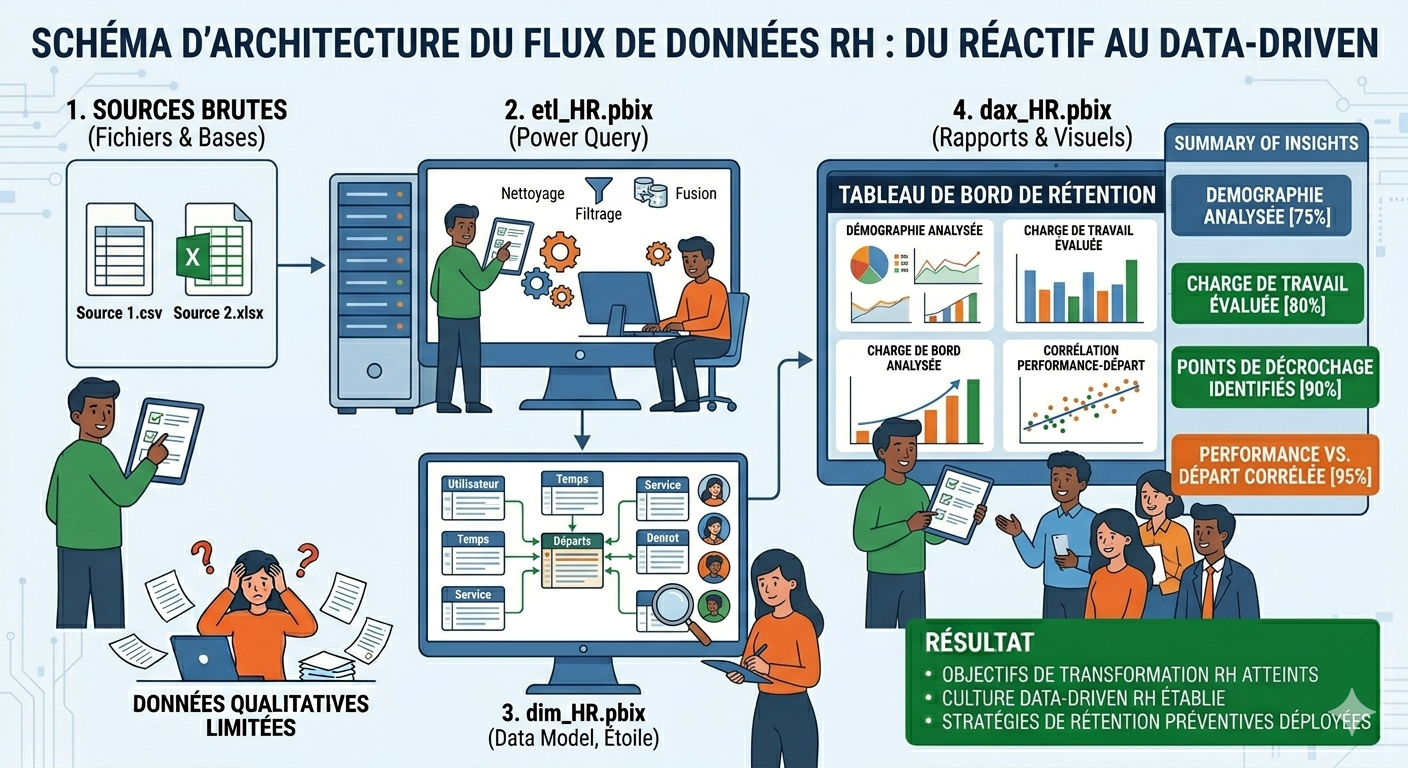
\includegraphics[width=0.8\textwidth]{figures/fig2_1_architecture.png.png}
    \caption{Flux de données et architecture modulaire}
    \label{fig:architecture}
\end{figure}

\section{Stratégie de Versioning et Git Workflow}
Le développement collaboratif a été orchestré via Git, permettant à chaque membre de travailler sur son axe de spécialisation sans interférer avec les autres :

\begin{itemize}
    \item \textbf{main :} Branche stable contenant la version de production validée.
    \item \textbf{feature/etl-pipeline :} Développement des flux M et nettoyage des sources.
    \item \textbf{feature/data-modeling :} Structuration des tables de faits et dimensions.
    \item \textbf{feature/kpi-logic :} Implémentation des formules DAX complexes.
    \item \textbf{feature/dashboard-design :} Travail sur l'ergonomie et les visuels.
\end{itemize}

Cette approche garantit une traçabilité complète des modifications et facilite l'intégration continue des nouveaux indicateurs.

\chapter{Conception Fine et Réalisation Technique}

\section{Pipeline ETL et Préparation des Données (etl\_HR.pbix)}
La phase ETL a été conçue pour transformer des données RH brutes et hétérogènes en un ensemble cohérent et prêt pour l'analyse.

\subsection{Transformations appliquées sous Power Query}
Les principales étapes de transformation incluent :
\begin{itemize}
    \item \textbf{Typage et Nettoyage :} Conversion des colonnes de salaire en entier et normalisation des noms de départements.
    \item \textbf{Gestion des valeurs nulles :} Pour les employés actifs, la date de sortie (\textit{ExitDate}) a été gérée dynamiquement pour permettre le calcul de l'ancienneté.
    \item \textbf{Segmentation (SalaryBand) :} Création d'une colonne conditionnelle classant les employés par tranches de salaire (Entry, Mid, Senior, Executive).
    \item \textbf{Ancienneté (Tenure\_Years) :} Calcul de la durée de présence en années à partir de la date d'embauche et de la date de sortie (ou aujourd'hui).
\end{itemize}

\begin{figure}[h]
    \centering
    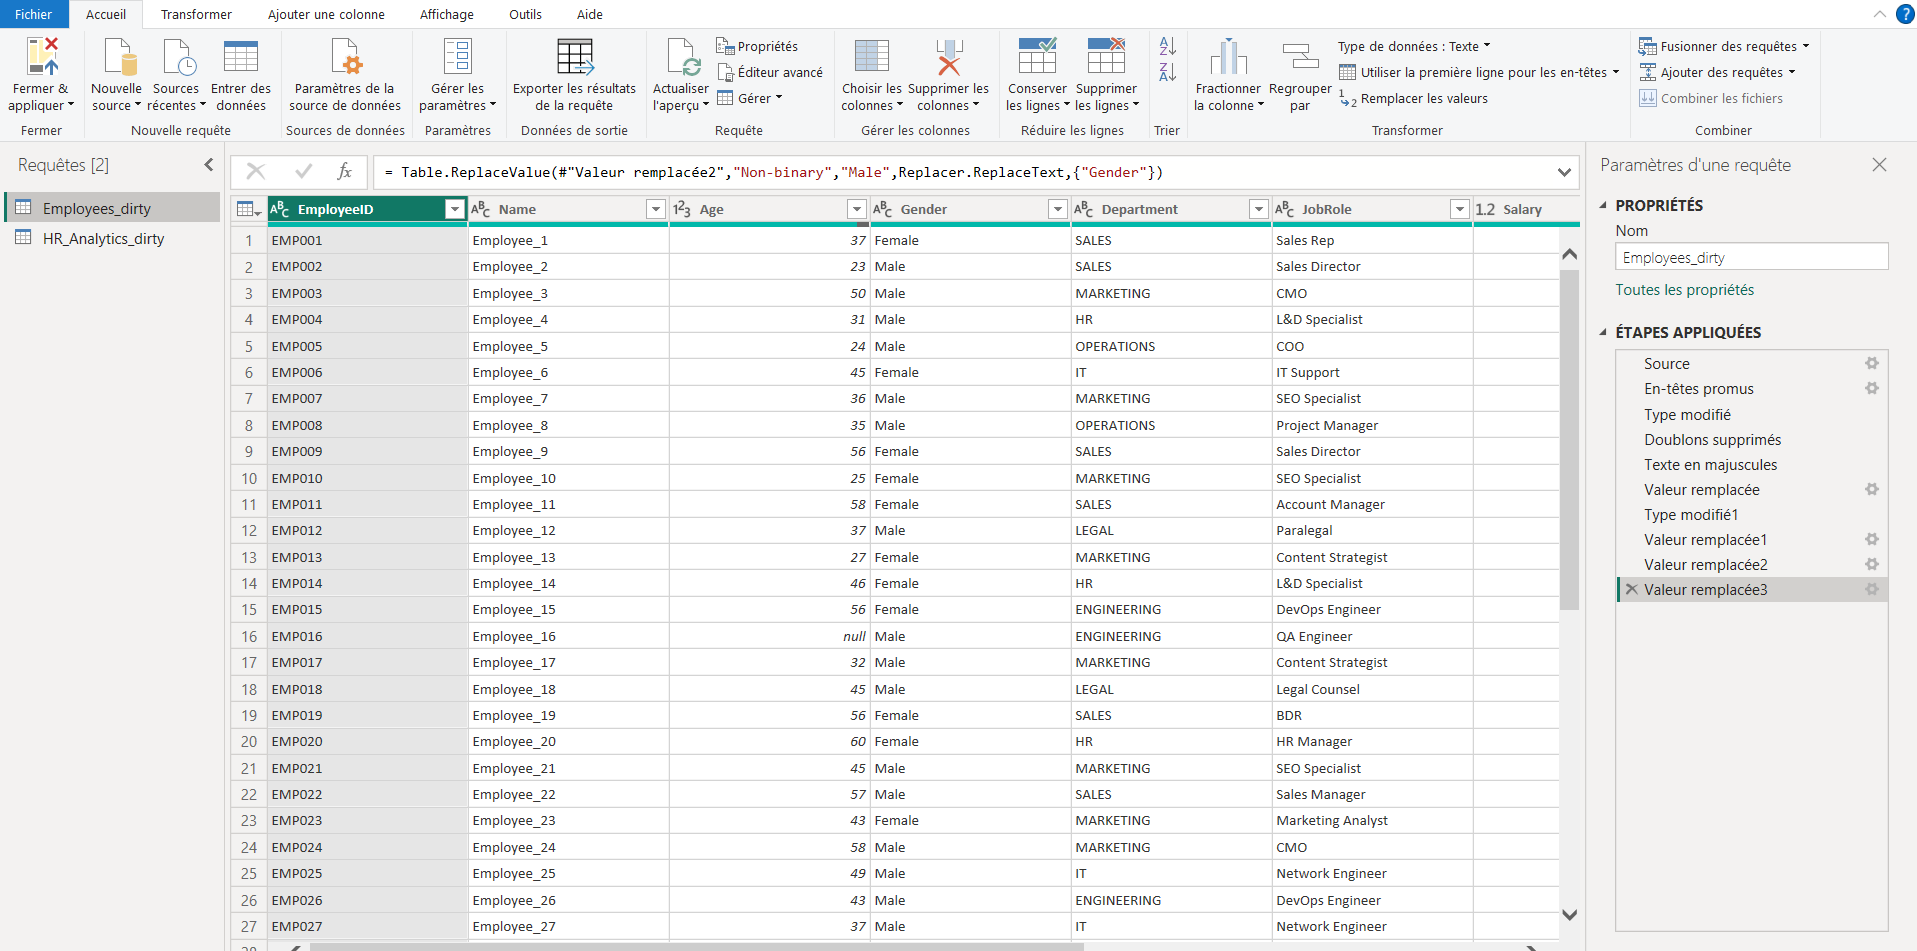
\includegraphics[width=0.8\textwidth]{figures/fig3_1_powerquery.png}
    \caption{Aperçu du pipeline de transformation Power Query}
    \label{fig:etl}
\end{figure}

\section{Modélisation Conceptuelle et Schéma en Étoile (dim\_HR.pbix)}
L'architecture du modèle repose sur un \textbf{Schéma en Étoile}, garantissant des performances optimales et une clarté analytique.

\subsection{Structure du modèle}
\begin{itemize}
    \item \textbf{FactHR (Table de faits) :} Centralise les mesures (Salaire, satisfaction, évaluation) et les clés étrangères vers les dimensions.
    \item \textbf{DimEmployee (Dimension) :} Attributs granulaires des collaborateurs (Âge, Genre, Rôle).
    \item \textbf{DimDepartment (Dimension) :} Nomenclature des pôles d'activité.
    \item \textbf{DimDate (Dimension) :} Calendrier dynamique pour les analyses temporelles.
\end{itemize}

\begin{figure}[h]
    \centering
    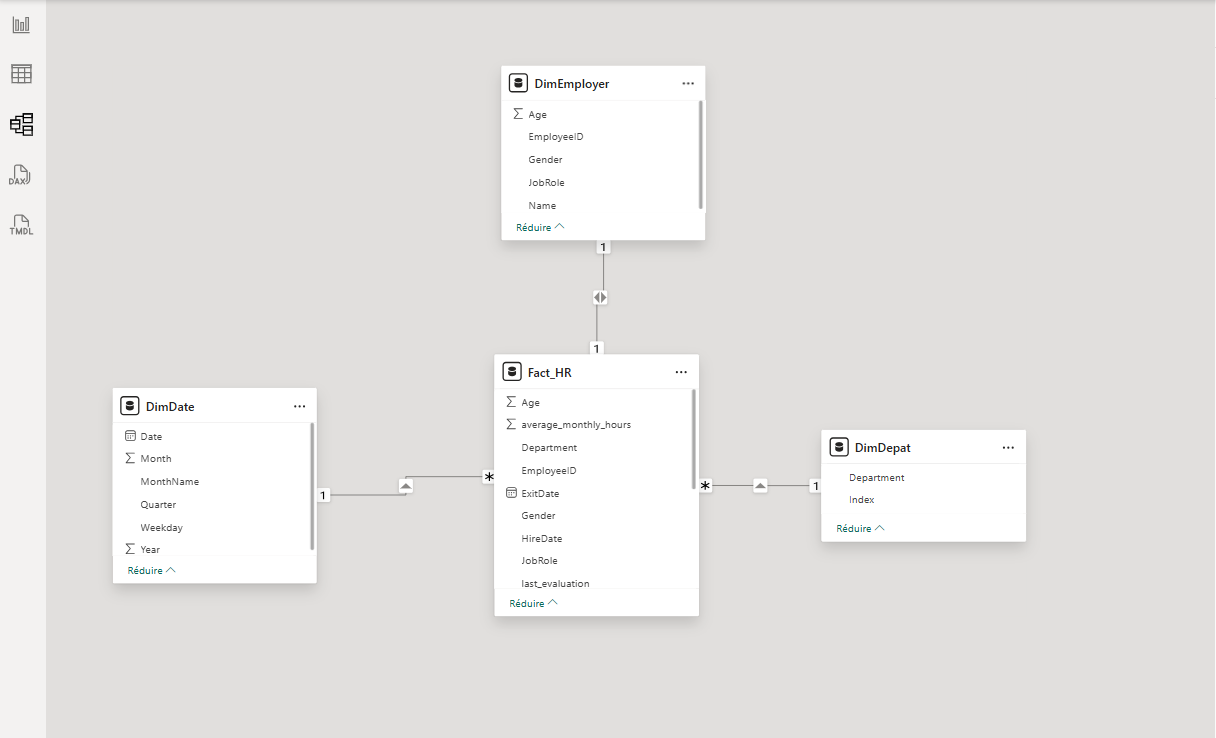
\includegraphics[width=0.9\textwidth]{figures/modele_etoile.png}
    \caption{Architecture du Schéma en Étoile finalisé}
    \label{fig:star_schema}
\end{figure}

\section{Développement des Métriques et Logique Analytique (dax\_HR.pbix)}
Le moteur DAX a été utilisé pour traduire les besoins métiers en indicateurs de performance (KPIs) dynamiques.

\subsection{Exemples de mesures DAX clés}
Nous avons implémenté des mesures avancées pour isoler les risques d'attrition :

\begin{itemize}
    \item \textbf{Attrition Rate :}
    \begin{lstlisting}[language=SQL]
Attrition Rate = 
DIVIDE(
    CALCULATE(DISTINCTCOUNT(FactHR[EmployeeID]), FactHR[left] = 1),
    [Total Employees], 0
)
    \end{lstlisting}
    
    \item \textbf{Overtime Risk Score :} Identifie les employés dépassant 220 heures mensuelles.
    \begin{lstlisting}[language=SQL]
Overtime Risk Score = 
CALCULATE(
    DISTINCTCOUNT(FactHR[EmployeeID]),
    FILTER(FactHR, FactHR[average_monthly_hours] > 220)
)
    \end{lstlisting}
\end{itemize}

\begin{figure}[h]
    \centering
    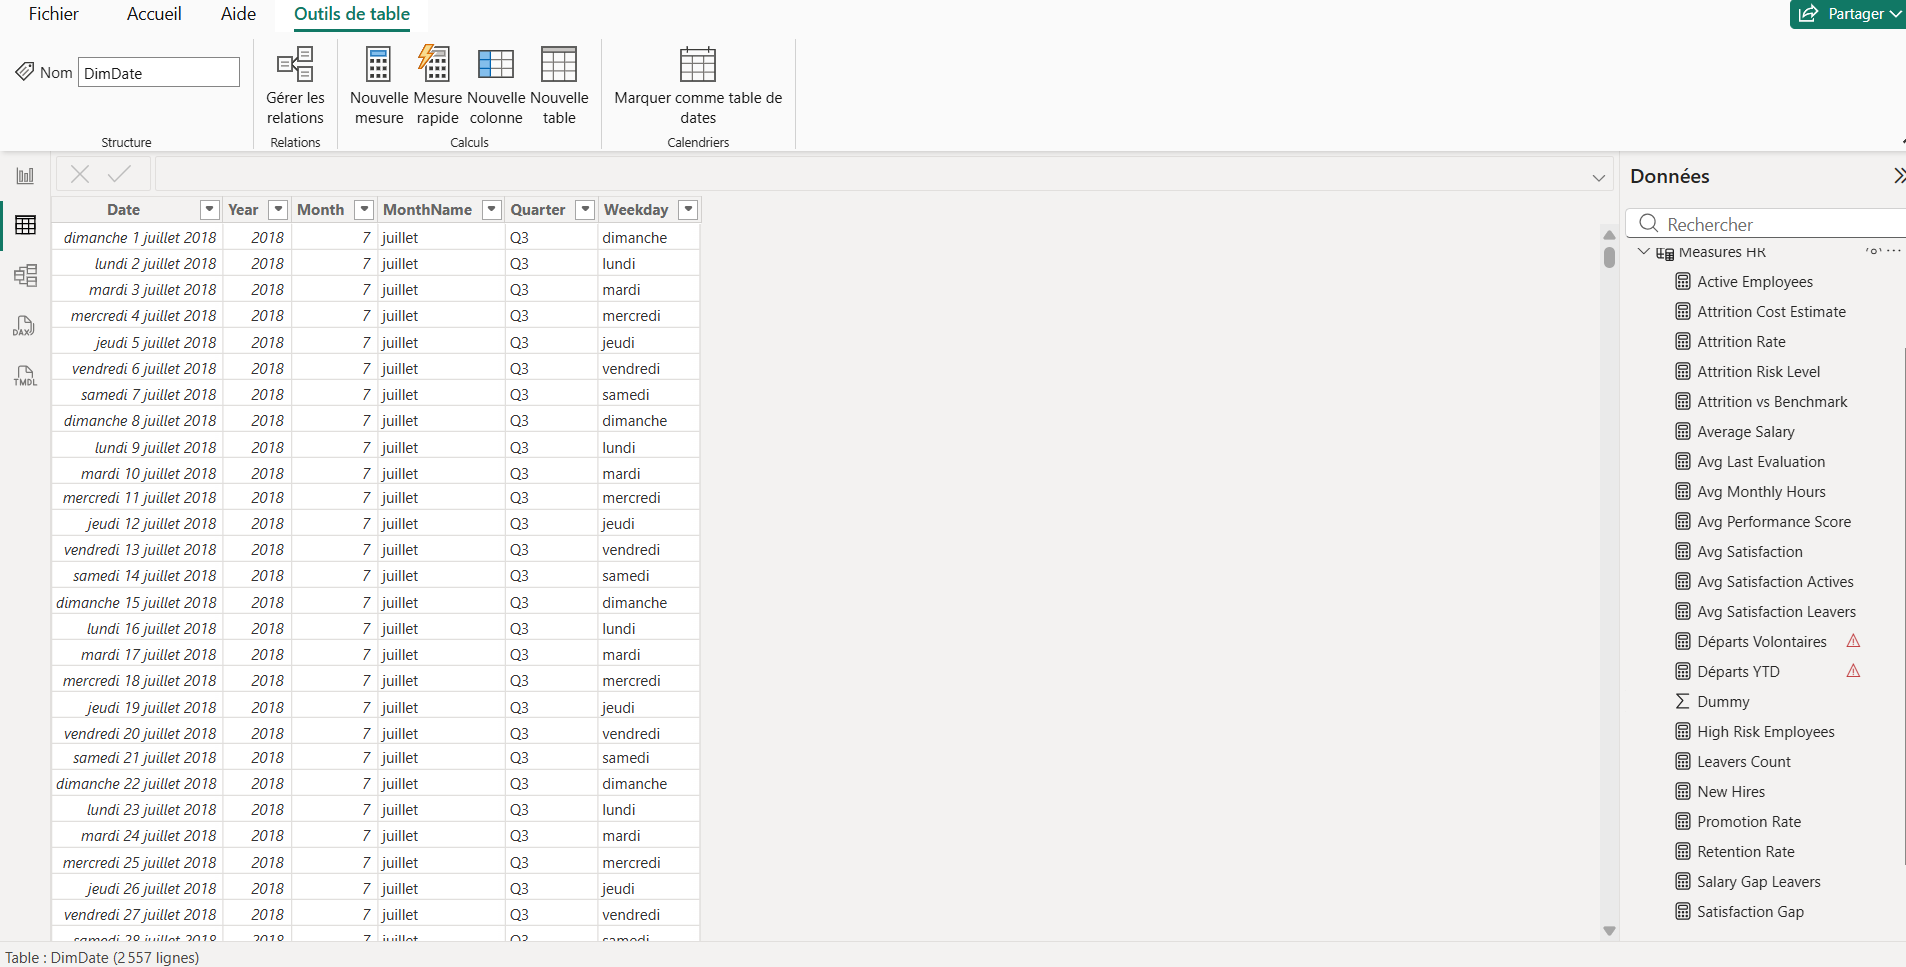
\includegraphics[width=0.8\textwidth]{figures/fig3_3_dax.png}
    \caption{Visualisation d'une mesure complexe dans Power BI Desktop}
    \label{fig:dax}
\end{figure}

\chapter{Processus ETL}

\section{Architecture du processus ETL}

Le processus ETL (Extraction, Transformation, Chargement) est la colonne vertébrale technique de tout système de Business Intelligence. Son rôle est de garantir que les données brutes issues des systèmes sources sont nettoyées, harmonisées et structurées selon le modèle dimensionnel défini précédemment. Pour ce projet \textit{HR Analytics}, le flux de données a été conçu pour transformer un fichier plat (CSV) en un ensemble de tables prêtes pour l'analyse multidimensionnelle.

L'architecture ETL adoptée se décompose en trois phases distinctes, chacune ayant des objectifs de qualité et d'intégrité rigoureux.

\section{Extraction et Nettoyage des données}

La phase d'extraction consiste à récupérer les données de base. Lors de cette étape, nous avons constaté que certaines variables étaient redondantes ou n'apportaient aucune valeur informative car elles présentaient une variance nulle (valeur identique pour tous les employés). 

Dans un souci d'optimisation des performances et de clarté, les opérations suivantes ont été réalisées :
\begin{itemize}
    \item \textbf{Suppression de colonnes inutiles :} Des variables telles que \textit{EmployeeCount}, \textit{StandardHours} et \textit{Over18} ont été écartées du modèle.
    \item \textbf{Gestion de l'intégrité :} Vérification de l'absence de doublons et de valeurs aberrantes (par exemple, des salaires négatifs ou des âges incohérents).
\end{itemize}

\section{Transformations et Logique métier}

C'est lors de la phase de transformation que les données prennent leur valeur sémantique. Les traitements appliqués sont variés et essentiels pour le calcul des KPIs.

\begin{figure}[h]
\centering
% espace réservé pour le diagramme du flux ETL
\caption{Diagramme de flux des transformations de données}
\end{figure}

Les principales transformations effectuées incluent :
\begin{itemize}
    \item \textbf{Codage catégoriel :} Transformation des variables textuelles en formats exploitables par les outils de calcul. La variable \textit{Attrition} a été convertie en format binaire (Oui = 1, Non = 0) pour permettre le calcul direct du taux d'attrition moyen. De même, la variable \textit{OverTime} a été numérisée.
    \item \textbf{Segmentation (Binning) :} Création de tranches d'âge et de tranches d'ancienneté pour faciliter les analyses de groupes (par exemple : [18-25], [26-35], etc.).
    \item \textbf{Normalisation des labels :} Harmonisation des noms de départements et des rôles pour éviter les discordances lors des regroupements.
\end{itemize}

\section{Chargement dans le modèle décisionnel}

La dernière étape consiste à charger les données transformées dans les tables respectives du schéma en étoile (\textit{Fact} et \textit{Dimensions}). Ce chargement est effectué de manière à respecter l'intégrité référentielle : les tables de dimensions sont chargées en premier pour générer les clés techniques, suivies par la table de faits. 

Le résultat final est un jeu de données "propre", cohérent et optimisé, permettant une interactivité fluide lors de la phase de visualisation, avec des temps de réponse minimaux même lors de filtrages complexes.

\chapter{Analyse et Visualisation}

\section{Conception des Tableaux de bord}

La visualisation des données est l'aboutissement du projet de Business Intelligence. Son but est de traduire des données complexes en informations visuelles intuitives pour soutenir la prise de décision. Pour l'analyse de l'attrition et de la performance, nous avons conçu un tableau de bord interactif structuré en plusieurs pages thématiques, permettant aux gestionnaires d'explorer les données à différents niveaux de granularité.

\begin{figure}[h]
\centering
% espace réservé pour la vue d'ensemble du dashboard (Page 1)
\caption{Vue d'ensemble du tableau de bord RH - Analyse de l'attrition}
\end{figure}

Le design a été guidé par les principes de la "Data Visualization" : utilisation de codes couleurs cohérents (rouge pour l'attrition positive, vert pour la stabilité), mise en avant des KPIs critiques en haut de page, et intégration de filtres dynamiques par département, genre et rôle professionnel.

\section{Analyse multidimensionnelle et Insights}

L'exploitation des tableaux de bord a permis de mettre en évidence plusieurs phénomènes structurants au sein de l'organisation. L'analyse ne se limite pas au constat du taux de départ, mais cherche à en comprendre les racines profondes.

\subsection{Analyse par Profil et Département}

L'un des premiers constats concerne la disparité entre les départements. Le département des \textit{Ventes} présente un taux d'attrition significativement plus élevé que celui de la \textit{Recherche et Développement}. Cela suggère des conditions de stress ou de pression sur les objectifs plus marquées dans ces fonctions.

\begin{figure}[h]
\centering
% espace réservé pour le graphique de l'attrition par département
\caption{Répartition du taux d'attrition selon les départements et les rôles}
\end{figure}

\subsection{L'impact des facteurs de travail}

L'analyse croisée des heures supplémentaires et de la satisfaction révèle un insight majeur : les employés effectuant des heures supplémentaires régulières ont un taux d'attrition deux fois supérieur à la moyenne. Ce facteur semble primer sur le niveau de rémunération pour une part importante des départs volontaires.

De plus, la distance domicile-travail apparaît comme un facteur d'érosion silencieux. Au-delà d'un certain seuil kilométrique, la probabilité de départ augmente de manière exponentielle, soulignant l'importance des politiques de télétravail ou de flexibilité géographique.

\section{Interprétation de la performance}

En parallèle de l'attrition, le tableau de bord permet d'évaluer la performance. Nous observons une corrélation positive entre le niveau d'implication (\textit{Job Involvement}) et la note de performance. Cependant, il est intéressant de noter que certains des employés les plus performants se situent également dans les segments à risque d'attrition, souvent par manque de perspectives de promotion ou d'équilibre vie-travail.

\begin{figure}[h]
\centering
% espace réservé pour le graphique corrélation performance vs attrition
\caption{Analyse de la relation entre performance et risque de départ}
\end{figure}

Ces résultats fournissent une base factuelle pour la direction des ressources humaines, leur permettant de cibler leurs actions de rétention non pas de manière uniforme, mais en fonction des facteurs de risque identifiés par le système BI.

\chapter{Conclusion et Perspectives}

\section{Synthèse du projet}

Le projet \textit{HR Analytics - Employee Attrition \& Performance} a permis de concevoir une solution de Business Intelligence complète, capable de transformer des données RH brutes en un outil d'aide à la décision stratégique. En suivant une méthodologie rigoureuse, nous avons franchi les étapes de l'analyse des besoins, de la modélisation dimensionnelle en étoile, du processus ETL et enfin de la visualisation interactive.

L'analyse a révélé que l'attrition n'est pas un phénomène aléatoire mais qu'elle est étroitement liée à des facteurs identifiables tels que la charge de travail (heures supplémentaires), l'équilibre vie-travail et la structure de rémunération. La mise en place de cet entrepôt de données offre désormais à l'organisation une vision claire et objective de son capital humain, permettant de passer d'une gestion intuitive à une gestion basée sur les faits.

\section{Limites et Recommandations}

Bien que robuste, le système actuel présente certaines limites inhérentes à la nature statique des données utilisées. Pour maximiser l'impact des résultats obtenus, nous recommandons à la direction des ressources humaines :
\begin{itemize}
    \item \textbf{Ciblage des politiques de rétention :} Mettre en place des programmes de bien-être spécifiques pour les départements à forte pression (Ventes) et revoir la politique des heures supplémentaires.
    \item \textbf{Flexibilité :} Encourager le télétravail pour les collaborateurs éloignés géographiquement afin de réduire l'attrition liée aux déplacements.
\end{itemize}

\section{Perspectives d'évolution}

Ce projet constitue une première étape solide vers une gestion mature des ressources humaines par les données. Plusieurs perspectives d'évolution peuvent être envisagées pour enrichir cette solution :

D'une part, l'intégration de nouvelles sources de données, telles que les données issues des réseaux sociaux d'entreprise ou les feedbacks qualitatifs des entretiens de sortie, permettrait d'affiner la compréhension des motifs psychologiques de départ.

D'autre part, la transition du \textit{Descriptive Analytics} vers le \textit{Predictive Analytics} représente l'évolution naturelle de ce système. L'implémentation de modèles de Machine Learning (tels que les forêts aléatoires ou les réseaux de neurones) permettrait de calculer un "score de risque de départ" individuel. Cette approche prédictive offrirait aux managers la possibilité d'intervenir en amont, par le biais d'actions de rétention personnalisées, avant même que la décision de départ ne soit formalisée par l'employé.


%-------------- Back Matter --------------
\chapter*{Bibliographie}
\addcontentsline{toc}{chapter}{Bibliographie}

\begin{enumerate}

    \item Ralph Kimball, Margy Ross. \textit{The Data Warehouse Toolkit: The Definitive Guide to Dimensional Modeling}, 3rd Edition, Wiley, 2013.

    \item Christian S. Jensen, Torben Bach Pedersen, Christian Thomsen. \textit{Multidimensional Databases and Data Warehousing}, Morgan \& Claypool, 2010.

    \item IBM HR Analytics Employee Attrition \& Performance Dataset, Kaggle, 
    \url{https://www.kaggle.com/datasets/pavansubhasht/ibm-hr-analytics-attrition-dataset}.

    \item Gartner. \textit{Magic Quadrant for Analytics and Business Intelligence Platforms}, 2024.

    \item Bernard Marr. \textit{Data-Driven HR: How to Use Analytics and Big Data to Drive Performance}, Kogan Page, 2018.

    \item William H. Inmon. \textit{Building the Data Warehouse}, 4th Edition, Wiley, 2005.

    \item Jiawei Han, Micheline Kamber, Jian Pei. 
    \textit{Data Mining: Concepts and Techniques}, 3rd Edition, Morgan Kaufmann, 2011.

    \item Thomas H. Davenport, Jeanne G. Harris. 
    \textit{Competing on Analytics: The New Science of Winning}, Harvard Business Review Press, 2007.

    \item Microsoft. \textit{Power BI Documentation and Learning Resources}, 2024. 
    \url{https://learn.microsoft.com/power-bi/}

    \item Oracle. \textit{Oracle Database Data Warehousing Guide}, Oracle Documentation, 2024. 
    \url{https://docs.oracle.com/en/database/}

    \item SAP. \textit{SAP Business Intelligence and Analytics Solutions}, SAP Documentation, 2024. 
    \url{https://www.sap.com/products/technology-platform/analytics.html}

    \item Society for Human Resource Management (SHRM). 
    \textit{People Analytics: Using Data to Improve Workforce Performance}, 2023. 
    \url{https://www.shrm.org/}

    \item Foster Provost, Tom Fawcett. 
    \textit{Data Science for Business: What You Need to Know about Data Mining and Data-Analytic Thinking}, O’Reilly Media, 2013.

    \item Tableau. \textit{Tableau Business Intelligence and Analytics Platform Documentation}, 2024. 
    \url{https://www.tableau.com/learn/training}

    \item Kaggle. \textit{HR Employee Attrition and Performance Analysis Projects and Resources}, 2024. 
    \url{https://www.kaggle.com/}

    \item Wes McKinney. \textit{Python for Data Analysis}, 3rd Edition, O’Reilly Media, 2022.

    \item Microsoft SQL Server. \textit{SQL Server Data Warehouse Documentation}, 2024. 
    \url{https://learn.microsoft.com/sql/}

    \item Tom White. \textit{Hadoop: The Definitive Guide}, 4th Edition, O’Reilly Media, 2015.

    \item Stephen Few. \textit{Information Dashboard Design: Displaying Data for At-a-Glance Monitoring}, 2nd Edition, Analytics Press, 2013.

    \item Deloitte. \textit{Global Human Capital Trends Report}, 2024. 
    \url{https://www2.deloitte.com/global/en/pages/human-capital/topics/human-capital-trends.html}

\end{enumerate}
\chapter*{Annexes}
\addcontentsline{toc}{chapter}{Annexes}

\section*{Annexe A : Description du Dataset}
Le dataset utilisé dans ce projet est le jeu de données IBM HR Analytics Employee Attrition \& Performance disponible sur Kaggle.  
Il contient des informations sur les employés telles que :
\begin{itemize}
    \item Âge
    \item Département
    \item Salaire mensuel
    \item Niveau d’éducation
    \item Satisfaction au travail
    \item Nombre d’années d’expérience
    \item Taux d’attrition
\end{itemize}

\section*{Annexe B : Technologies Utilisées}
Les principales technologies utilisées dans ce projet sont :
\begin{itemize}
    \item Python
    \item Pandas
    \item NumPy
    \item SQL Server
    \item Power BI
    \item Jupyter Notebook
\end{itemize}

\section*{Annexe C : Exemple de Requête SQL}
\begin{verbatim}
SELECT Department,
       AVG(MonthlyIncome) AS AverageSalary
FROM Employees
GROUP BY Department;
\end{verbatim}

\section*{Annexe D : Captures d’Écran}
Cette section contient :
\begin{itemize}
    \item Les tableaux de bord Power BI
    \item Les visualisations analytiques
    \item Les résultats des analyses RH
\end{itemize}

\section*{Annexe E : Objectifs du Projet}
Les principaux objectifs du projet sont :
\begin{itemize}
    \item Construire un Data Warehouse RH
    \item Analyser les performances des employés
    \item Étudier les facteurs d’attrition
    \item Faciliter la prise de décision grâce à la Business Intelligence
\end{itemize}

\end{document}
